% Created 2022-02-14 lun 19:39
% Intended LaTeX compiler: pdflatex
\documentclass[11pt,a4paper]{article}

\usepackage[utf8]{inputenc}
\usepackage[T1]{fontenc}
\usepackage[spanish]{babel}
\usepackage{amsmath}
\usepackage{amsfonts}
\usepackage{fancyhdr}
\usepackage{amssymb}
\usepackage[font=scriptsize,labelfont=bf]{caption}
\usepackage{lmodern}
\usepackage{xcolor} 
\usepackage{mdframed}
\usepackage{wrapfig}
\usepackage{multirow} 
\usepackage{lipsum}
\usepackage{multicol} 
\usepackage{scrextend} 
\usepackage{tikz}
\usetikzlibrary{positioning}
\usepackage{float}
\usepackage{graphicx}
\usepackage{tikzpagenodes}
\usepackage[absolute]{textpos} 
\usepackage{colortbl}
\usepackage{array}
\usepackage[hidelinks]{hyperref}
\usepackage[makeroom]{cancel}
\usepackage{eso-pic}
\usepackage[a4paper,left=3cm,right=2cm,top=2.5cm,bottom=2.5cm]{geometry}
\usepackage[final]{pdfpages}
\usepackage{float}
\usepackage{fancyhdr}
\pagestyle{fancy}
\fancyhf{}
\lhead{Sistemas electrónicos}
\rhead{Jorge Benavides Macías}
\rfoot{\thepage}
\renewcommand{\headrulewidth}{0.4pt}% Default \headrulewidth is 0.4pt
\setlength{\headheight}{16pt}
\setlength{\parskip}{1em}
\setlength{\parindent}{0em}
\definecolor{my_blue}{RGB}{0, 46, 93}
\definecolor{my_white}{RGB}{255, 255, 255}
\definecolor{Prune}{RGB}{0,46,93}

\newcommand*{\dummypic}[4]{%
\setlength{\fboxsep}{0pt}%
\begin{minipage}[t][0.2\textwidth][c]{0.25\textwidth}
\centering \includegraphics[#1]{#2}
\caption{#3}
\label{#4}
\end{minipage}%
}

\datosportada{Grado en ingeniería en electrónica, robótica y mecatrónica}{Fundamentos de robótica}{Ejercicios}{Transformadas homogéneas. Relaciones entre sistemas de coordenadas}{Tarea \# 1}{Ejercicios de sistemas de coordenadas resueltos con MATLAB}{images/brazo.png}{2021-2022}{Jorge Benavides Macías}

\hypersetup{
 pdfauthor={Jorge Benavides M.},
 pdftitle={Transformadas homogéneas. Relaciones entre sistemas de coordenadas},
 pdfkeywords={},
 pdfsubject={Fundamentos de robótica},
 pdfcreator={Overleaf}, 
 pdflang={Spanish}}
\begin{document}

\portada
\newpage

\begin{figure}[H]
    \centering
    \includegraphics[scale=0.75]{images/diagram-20220310.pdf}
    \caption{\textbf{Grafo de las relaciones entre los sistemas de coordenadas.}}
\end{figure}

\textbf{Nota$_1$:} B respecto de A es ATB, giros o traslaciones respecto a un mismo sistema se describen con subíndices, por ejemplo, $^{C_1}T_{C}$ en matlab se escribe como C1TC.

\textbf{Nota$_2$:} He añadido dos funciones para realizar las rotaciones y las traslaciones, al final de este documento recojo el código utilizado, el único objetivo de usarlas es simplificar el proceso de análisis y dejar el código más claro Para usarlas deben añadirse al Path de MATLAB.

\begin{matlabcode}
CTO = [0 1 0 1;  1 0 0 10; 0 0 -1 9; 0 0 0 1]; 
CTB = [1 0 0 -10; 0 -1 0 20; 0 0 -1 10; 0 0 0 1]; 
\end{matlabcode}

\begin{enumerate}
    \item \textbf{¿Cuál es la posición del centro del cubo con respecto al sistema de coordenadas de la base?}
    
    Para obtener esta transformación debemos seguir el camino inverso desde ${B}$ a ${O}$ por lo que hacemos uso de las matrices $^CT_B$ y $^CT_O$. Como nuestro objetivo es conseguir $^BT_O$, debemos invertir $^CT_B$ \rightarrow $^BT_C$ y multiplicarlo por $^CT_O$. Las operaciones que tenemos que realizar son:
    \[^BT_O = \left({}^CT_B\right)^{-1} * {}^CT_O\]
    
\begin{matlabcode}
BTO = inv(CTB)*CTO
\end{matlabcode}
\begin{matlaboutput}
BTO = 4x4    
     0     1     0    11
    -1     0     0    10
     0     0     1     1
     0     0     0     1
\end{matlaboutput}
    
    \item \textbf{Suponer que el cubo se encuentra dentro del alcance del brazo y que este dispone de un sistema de  referencia en su efector final \{H\}, ¿Cuál es la matriz de orientación de dicho efector final, referida al  sistema de referencia de la base, si se requiere que la pinza del robot se alinee con el eje Y del cubo (esto implica que el eje Y de ambos sistemas estén alineados) y al mismo tiempo lo coja desde arriba (la garra hacia abajo, y, por tanto, su eje Z hacia abajo)?}
    
    Como el actuador debe estar en la posición del objeto, es un giro de 180 grados respecto a ``y'', además hay que usar la matriz de transformación $^BT_O$ para pasar de la base al objeto y después girar dicha base para obtener el eje z hacia abajo. La operación resultante es:
    \[{}^BT_H = {}^BT_O * {}^OT_H \]
    
    Donde ${}^OT_H$ representa la rotación de 180 grados respecto ``y''.
    
\begin{matlabcode}
OTH = rot('y',180);
BTH = BTO*OTH
\end{matlabcode}
\begin{matlaboutput}
BTH = 4x4    
         0    1.0000         0   11.0000
    1.0000         0   -0.0000   10.0000
   -0.0000         0   -1.0000    1.0000
         0         0         0    1.0000
\end{matlaboutput}
    
    \item \textbf{Desgraciadamente, después de que se ha colocado el equipo y se han tomado estos sistemas de  coordenadas, alguien gira la cámara 90° respecto del eje Z de la cámara. ¿Cuál es la localización de  la cámara con respecto al sistema de coordenadas de la base del robot?}
    
    Este apartado es muy similar al anterior, un giro respecto a ``z'' multiplicada por una matriz de transformación, salvo con la diferencia de que usamos la inversa de esta última, el motivo es porque en nuestro grafo conocemos $^CT_B$ y nuestro interés es por $^BT_C$ así que debemos invertirla y obtenemos las siguientes operaciones.
    
    \[^BT_{C_1} = \left({}^CT_B\right)^{-1} * {}^CT_{C_1}\]
    
\begin{matlabcode}
CTC1 = rot('z',90);
BTC1 = inv(CTB)*CTC1
\end{matlabcode}
\begin{matlaboutput}
BTC1 = 4x4    
    0.0000   -1.0000         0   10.0000
   -1.0000   -0.0000         0   20.0000
         0         0   -1.0000   10.0000
         0         0         0    1.0000
\end{matlaboutput}
    
    \item \textbf{Después de que haya calculado la respuesta a la pregunta anterior, la misma persona giró el objeto  90° respecto del eje x del objeto y lo trasladó cuatro unidades de distancia a lo largo del eje y girado.  Calcular la localización del objeto con respecto al sistema de coordenadas de la base del robot.}
    
    Este apartado es muy parecido a los anteriores, pero cuenta con un desplazamiento, como hemos visto en la teoría, ``una rotación + un desplazamiento'' no es igual a un ``desplazamiento + una rotación''; hay que seguir perfectamente los movimientos que indica el enunciado, primero se rotan 90 grados respecto al eje ``x'' siendo este un eje móvil y luego se desplaza 4 unidades en la dirección ``y''. Además, hay que multiplicarla por una matriz de transformación para ponerla respecto a la base del robot.
    
     \[^BT_{O_1} = {}^BT_O * {}^OT_{O_1}\]
    
\begin{matlabcode}
OTO1 = rot('x',90)*move(0,4,0);
BTO1 = BTO*OTO1
\end{matlabcode}
\begin{matlaboutput}
BTO1 = 4x4    
         0    0.0000   -1.0000   11.0000
   -1.0000         0         0   10.0000
         0    1.0000    0.0000    5.0000
         0         0         0    1.0000
\end{matlaboutput}
    
    \item \textbf{En las mismas circunstancias anteriores, calcular la localización del objeto con respecto al sistema de  coordenadas de la cámara girada.}
    
    Este apartado tiene como objetivo buscar un nuevo camino en el grafo y mediante las distintas transformaciones pasar de un sistema de referencia a otro. Nuestro objetivo es representar la matriz de transformación del objeto$_1$ respecto la cámara$_1$, una de las posibilidades es:
    
    \[^{C_{1}}T_{O_1} = \left({}^CT_{C_1}\right)^{-1}*{}^CT_O*{}^OT_{O_1}\]
    
\begin{matlabcode}
C1TO1_1 = inv(CTC1)*CTO*OTO1
\end{matlabcode}
\begin{matlaboutput}
C1TO1_1 = 4x4    
    1.0000    0.0000   -0.0000   10.0000
    0.0000   -0.0000    1.0000   -1.0000
         0   -1.0000   -0.0000    5.0000
         0         0         0    1.0000

\end{matlaboutput}

    \item \textbf{Considerar otra secuencia de transformaciones homogéneas que resuelva el punto anterior.}
    
\begin{matlabcode}
C1TO1_2 = inv(BTC1)*BTH*inv(OTH)*OTO1
\end{matlabcode}
\begin{matlaboutput}
C1TO1_2 = 4x4    
    1.0000    0.0000   -0.0000   10.0000
    0.0000   -0.0000    1.0000   -1.0000
         0   -1.0000   -0.0000    5.0000
         0         0         0    1.0000

\end{matlaboutput}
\begin{matlabcode}
C1TO1_3 = inv(BTC1)*inv(CTB)*CTO*OTO1
\end{matlabcode}
\begin{matlaboutput}
C1TO1_3 = 4x4    
    1.0000    0.0000   -0.0000   10.0000
    0.0000   -0.0000    1.0000   -1.0000
         0   -1.0000   -0.0000    5.0000
         0         0         0    1.0000

\end{matlaboutput}

\textbf{Representar todos los sistemas descritos en los apartados anteriores.}

\begin{matlabcode}
view(80,45);
grid on
Base =[1 0 0 0;0 1 0 0; 0 0 1 0; 0 0 0 1];
createFRAME(Base,'b','Base',1);
createFRAME(CTB,'r','CTB',1);
createFRAME(CTO,'r','CTO',1);
createFRAME(BTO,'r','BTO',1);
createFRAME(BTH,'m','BTH',1);
createFRAME(BTC1,'g','BTC1',1);
createFRAME(BTO1,'k','BT01',1);
createFRAME(C1TO1_1,'c','C1TO1_1',1);
\end{matlabcode}
\begin{figure}[H]
    \centering
    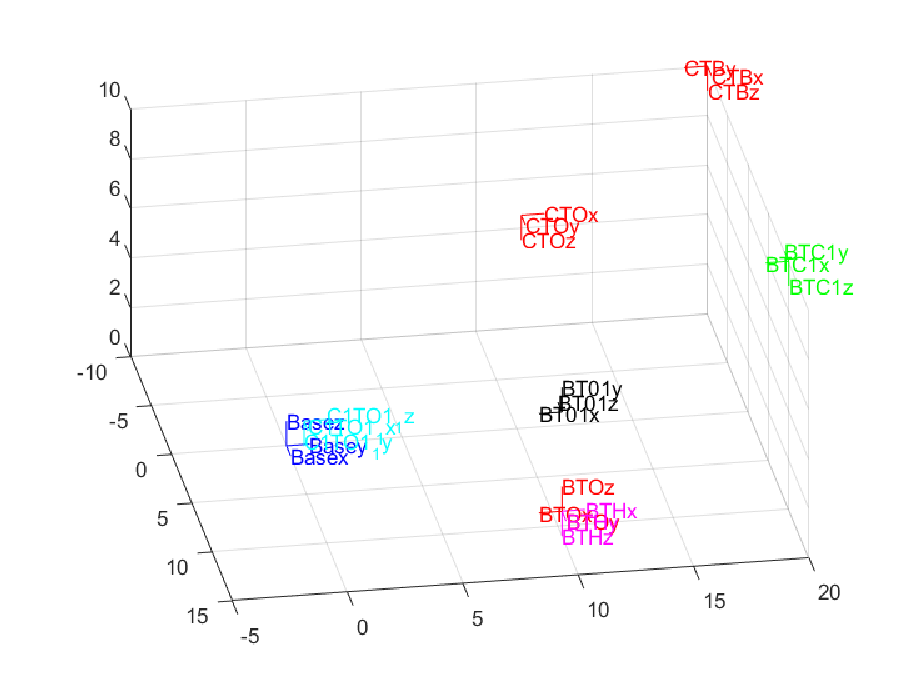
\includegraphics[scale=0.85]{images/figure_0.eps}
\end{figure}
\end{enumerate}


\textbf{Función rotación - rot()}
\begin{matlabcode}
function matrix_rot = rot(axis,angle)
sym al 'real';
sym be 'real';
sym ga 'real';
angle = deg2rad(angle);
switch axis
 case 'x'
  ga = angle;
  matrix_rot = [1 0 0 0; 0 cos(ga) -sin(ga) 0; 0 sin(ga) cos(ga) 0;0 0 0 1];
 case 'y'
  be = angle;
  matrix_rot = [cos(be) 0  sin(be) 0; 0 1 0 0; -sin(be) 0 cos(be) 0;0 0 0 1];
 otherwise
  al = angle;
  matrix_rot = [cos(al) -sin(al) 0 0; sin(al) cos(al) 0 0; 0 0 1 0; 0 0 0 1];
end
end
\end{matlabcode}

\textbf{Función desplazamiento - move()}
\begin{matlabcode}
function matrix_move = move(x,y,z)
matrix_move = [1 0 0 x;0 1 0 y; 0 0 1 z; 0 0 0 1];
end
\end{matlabcode}
\end{document}